%Question 3
\begin{enumerate}
	
	\item{
	%Part a
	\text{ }
		\begin{figure}[H]
		\begin{center}
		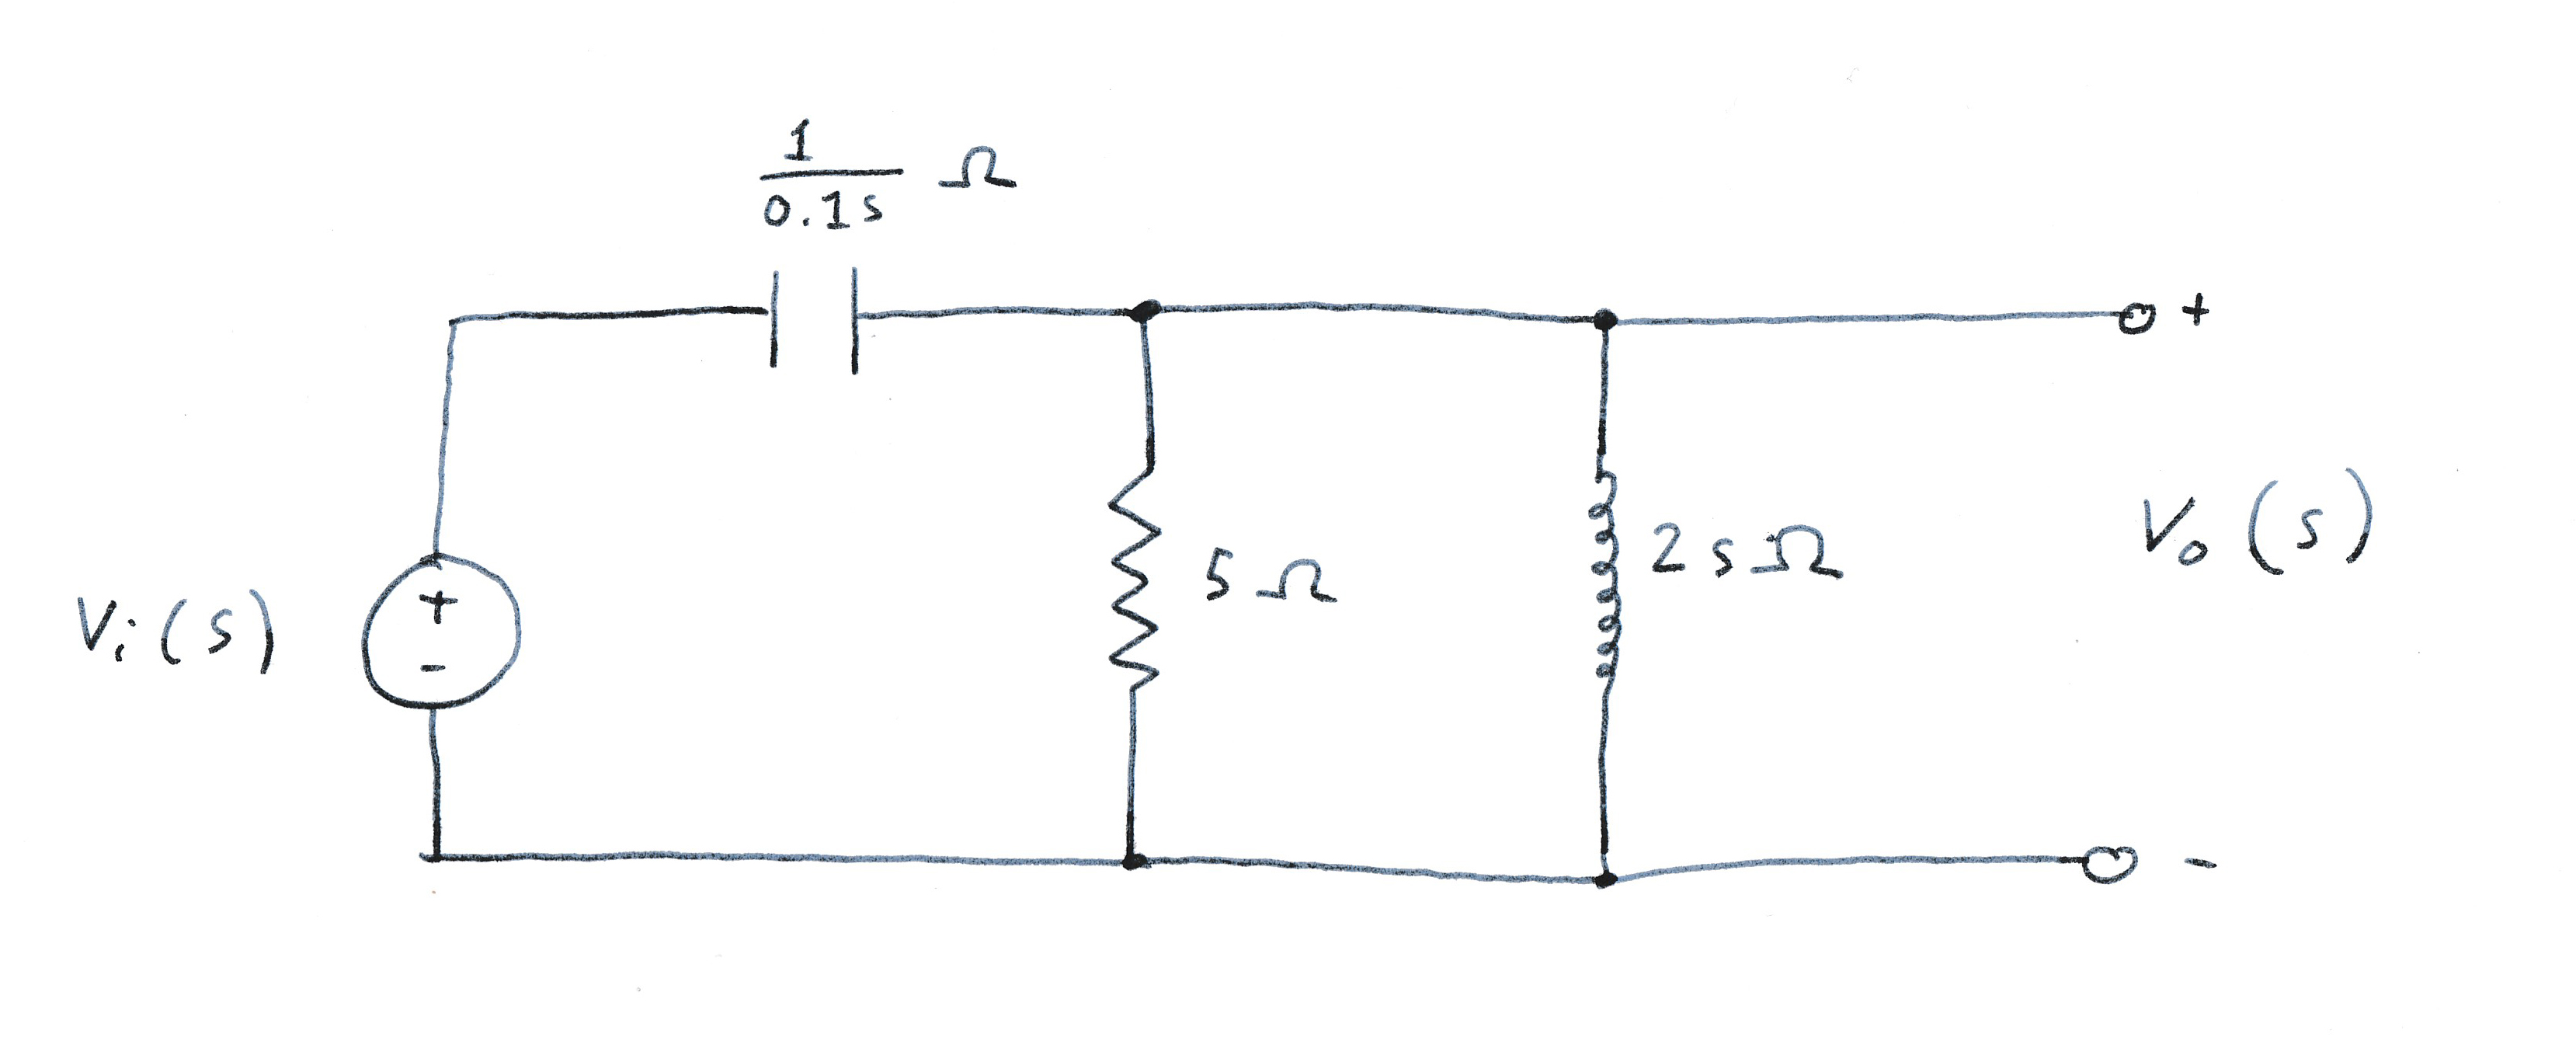
\includegraphics[scale=0.75]{3a.JPG}
		\end{center}
		\end{figure}
		\begin{align*}
		Z_{R||L} &= (\frac{1}{5} + \frac{1}{2s})^{-1}\\
		&= (\frac{2s+5}{10s})^{-1}\\
		&= \frac{10s}{2s+5}\\
		\implies H(s) &= \frac{V_o(s)}{V_i(s)}\\
		&= \frac{z_{R||L}}{Z_{R||L} + Z_C}\\
		&= \frac{\dfrac{10s}{2s+5}}{\dfrac{10s}{2s+5} + \dfrac{10}{s}}\\
		&= \frac{\dfrac{10s}{2s+5}}{\dfrac{10s^2+20s+50}{2s^2+5s}}\\
		&= \frac{s^2}{s^2+2s+5}
		\end{align*}
	}
	\item{
	%Part b
		Using phasor analysis:
		\begin{align*}
		V_o &= V_i \cdot \frac{\left((\dfrac{1}{R} + \dfrac{1}
		{j \omega L}\right)^{-1}}{\left(\dfrac{1}{R} + \dfrac{1}
		{j \omega L}\right)^{-1} + \dfrac{1}{j \omega C}}\\
		&= 10 \angle 0\degree \cdot \frac{\left( \dfrac{1}{5} + 
		\dfrac{1}{40j} \right)^{-1}}{\left( \dfrac{1}{5} + 
		\dfrac{1}{40j} \right)^{-1} + \dfrac{1}{2j}}\\
		&= 10.075 \angle 5.78\degree \;V
		\end{align*}
		This means that the steady state response for the 
		system when $v_i(t) = 10\cos{(20t)}$ is $v_o(t) = 
		10.075 \cos{(20t + 5.78\degree)}\;V$
	}
\end{enumerate}